% REMEMBER: You must not plagiarise anything in your report. Be extremely careful.

\documentclass{l4proj}

    
%
% put any additional packages here
\usepackage{siunitx}
\usepackage{float}
\usepackage{amsmath}
%

\begin{document}

%==============================================================================
%% METADATA
\title{Using Deep Learning to predict overall survival times for breast cancer from H\&E stained whole slide biopsy images}
\author{Anirbit Ghosh}
\date{September 14, 2022}

\maketitle

%==============================================================================
%% ABSTRACT
\begin{abstract}
    Current pathological practice to diagnose malignancy involves the manual identification and annotation of the extent of cancerous tumour cells in a biopsy slide image by a trained pathologist. This process is highly resource intensive and is subject to the interpretation variability between different readers leading to inconsistent outcomes. Therefore a Deep Learning based automated cancer detection system which can accurately and robustly identify the extent of malignancy from the digital whole slide image would be a highly desirable and potentially industry changing advancement. The subsequent step after the initial cancer diagnosis requires vast amounts of the patient's clinical data to be collected and processed in order to deliver a survival time prediction. The clinical data required to produce a survival time model for a patient ranges from general health and quality of life measures to specific characteristics of the malignant areas which must be extracted manually by pathologists. Given the sensitive nature of a cancer diagnosis in the first place it is often of essence to avoid putting patients through extensive diagnostic tests and data collection only to deliver potentially worse news with the survival time prognosis. Biopsy slide images hold a plethora of cellular level and structural information which can very effectively help understand the exact nature of malignancy. However, manually analyzing whole slide images to extract useful features is extremely expensive in terms of time and storage due to the sheer size of these images. Thus, augmenting the Deep Learning based cancer detection system to automatically extract useful features from the digital biopsy images can aid in characterizing cancer severity and giving a survival time estimate without the need of vast amounts of clinical data. The biggest problem in creating this system is the lack of annotated patient biopsy data that is publicly available, which makes effectively training a network to automatically detect malignant tissue extremely challenging. In this project, I proposed training a deep neural network on the Camelyon 16 data, which is a collection of 170 weakly annotated lymph node whole slide images from breast cancer patients. Breast cancer frequently metastasizes to axillary lymph nodes which makes them a good prognostic factor of breast cancer severity. The data contained 70 metastatic and 100 non-metastatic whole slides giving a good balance of positive and negative samples to train the network to accurately segment cancerous cells from a given tissue image. This process was a very unusual approach as there is no existing literature verifying the validity of using a network trained on breast metastasis found in lymph node tissue to detect malignancy in breast tissue. The different tissue composition posed a significant risk of complete network failure. However, the results showed surprisingly accurate and reasonable outcomes indicating that metastasis characterization transfers across multiple tissue types. The survival model was then generated using whole slide images of patients available on TCGA by processing their biopsies through the trained network and extracting features to characterize malignancy levels. The generated features were used as a heuristic in conjunction with each patient's predicted survival times (from associated clinical data) to generate a Cox Proportional-hazard model which is a regression model that can generates a survival time for a given heuristic level.  
    
\end{abstract}

%==============================================================================

% EDUCATION REUSE CONSENT FORM
% If you consent to your project being shown to future students for educational purposes
% then insert your name and the date below to  sign the education use form that appears in the front of the document. 
% You must explicitly give consent if you wish to do so.
% If you sign, your project may be included in the Hall of Fame if it scores particularly highly.
%
% Please note that you are under no obligation to sign 
% this declaration, but doing so would help future students.
%
\def\consentname {Anirbit Ghosh} % your full name
\def\consentdate {20 March 2022} % the date you agree
%
\educationalconsent


%==============================================================================
\tableofcontents

%==============================================================================
%% Notes on formatting
%==============================================================================
% The first page, abstract and table of contents are numbered using Roman numerals and are not
% included in the page count. 
%
% From now on pages are numbered
% using Arabic numerals. Therefore, immediately after the first call to \chapter we need the call
% \pagenumbering{arabic} and this should be called once only in the document. 
%
% The first Chapter should then be on page 1. You are allowed 40 pages for a 40 credit project and 20 pages for a 
% 20 credit report. This includes everything numbered in Arabic numerals (excluding front matter) up
% to but excluding the appendices and bibliography.
%
% You must not alter text size (it is currently 10pt) or alter margins or spacing.
%
%
%==================================================================================================================================
%
% IMPORTANT
% The chapter headings here are **suggestions**. You don't have to follow this model if
% it doesn't fit your project. Every project should have an introduction and conclusion,
% however. 
%
%==================================================================================================================================
\chapter{Introduction}

% reset page numbering. Don't remove this!
\pagenumbering{arabic} 

\section{Motivation}
With a global estimate of 18 million cases [1] of cancer diagnosed each year, as of 2020, female breast cancer has become the most common contributor making up over 12.5\% [2] of all cases of which 684,996 [3] cases were fatal making it the fifth leading cause of death. However, with an average 75\% 10-year survival rate across all stages of breast cancer [4], it shows the best prospects for generally being the most curable form provided an early diagnosis followed by appropriate and timely treatment. This constitutes the rationale for focusing this dissertation on improving the efficiency of breast cancer diagnosis and prognosis prediction. 

A biopsy is the only definitive way of diagnosing breast cancer. Traditionally a trained pathologist would be required to manually inspect a biopsied tissue sample and identify potential areas  abnormal, malignant cell growth. Subsequently an oncologist would use this pathology report to determine the patient's prognosis in terms of likelihood of recovery and survival chance which guides the course of treatment. Classical prognosis prediction  relies on population-level estimates by comparing a patient's case to previously documented similar cases based on cancer site, tumour grade, cancer stage and certain cellular markers. As every patient's cancer manifests uniquely, this technique is further supplemented by collecting the individual patient's clinical and quality of life information combined with several test results of multiple bio-markers. This complete diagnostic workflow is not only time consuming but also highly subjective and non-reproducible due to vast amount of data required to characterize each patient's condition and the manual effort required to produce and interpret that data.

If the delay between tissue collection, diagnosis and subsequent prognosis prediction could be minimized, it would allow patients to receive the appropriate treatment much quicker which can increase the likelihood of recovery in particularly time sensitive cases. Furthermore, reducing human involvement in the diagnostic procedure can eliminate interpretation variability making diagnoses more consistent and robust. As severe as it maybe, this will allow patients to be more confident in their first prognosis and eliminate the need to get a second opinion which in most cases serves as an unnecessary delay to starting the much needed treatment which could help increase their survival prospects. 


\section{General problem and our hypothesis}
The biopsied sample of breast tissue used in the diagnostic process is an exact characterization of the patient's individual condition. The structural and cellular level information obtained from biopsies is very valuable in understanding the extent and severity of cancer. A digital representation of the biopsied tissue can be obtained in the form a whole slide image (WSI), which is a high resolution, multi-level replication of the stained tissue as observed under a microscope at varying zoom levels. These digital slide images can be used in an automated cancer diagnostic system by treating the detection of malignant cells in the image as a classification problem. 

The general problem we are attempting to solve is to utilize digital whole slide images of biopsied tissue to automate the diagnosis of breast cancer without requiring manual annotation of tissue slides by pathologists. Furthermore, we are attempting to estimate the patient's prognosis in terms of an overall survival time by utilizing information extracted from the whole slide image, thereby eliminating the dependence on extensive clinical data collection and analysis. 

This paper proposes a supervised learning model which will be trained with patches of breast cancer whole slide images to learn how to perform slide level classification of malignant and benign tissue. Subsequently, we develop and extract some image-based features from the segmented whole slide images to predict an estimate for the survival time of the given patient. 



\section{Aim}
This project aims to investigate the viability of deep-learning based automated breast cancer diagnosis and corresponding survival time  prediction only using digital slide images of the affected tissue. We are trying to minimize or potentially eliminate the requirement of manual human intervention and vast amounts of clinical data in the diagnostic process. The project will achieve this by performing the following tasks:

\begin{itemize}
    \item
    elaborate the idea of automated cancer detection from whole slide images and describe the problem of inferring an estimated disease prognosis from a single slide image. 
    \item 
    prepare a training dataset with fixed size patches of whole slide images of breast tissue samples along with patch-level annotations for malignancy or benignity. The dataset must be standardized to eliminate any impact of human variability involved in the preparation of tissue slides collected from various sources.
    \item
    implement and train a supervised learning based deep convolutional neural network that can learn to distinguish between malignant and benign breast tissue. It will accept patches of a whole slide image and output a fully segmented whole slide image showing areas of malignancy.
    \item
    develop and extract a feature metric from the segmented whole slide image to quantify and characterize the nature of breast cancer in a given tissue slide. Using this metric, generate a statistical model to predict a proportional survival time for any given case. 
    \item
    evaluate the performance of the cancer detection network against clinically annotated ground truth samples. Measure accuracy of survival time prediction against available clinical data and infer validity of exclusively using whole slide images in delivering disease prognosis. 
\end{itemize}

%==================================================================================================================================
\chapter{Background}

\section{Whole Slide Images}
\subsection{Slide preparation}
Biopsied tissue blocks are sliced into thin sections and mounted on glass slides. For cancer diagnosis, these tissue slides are generally stained with a Hematoxylin and Eosin dye which has been proven (\textit{\cite{Bancroft2013}}) to exhibit selective affinity for specific cellular artifacts. Stained regions are more prone to absorbing light making them more prominently visible under illumination in a microscopy. In breast tissue, the Hematoxylin component stains the nuclei of cells in a blue colour as it binds to acidic structures, particularly RNA and DNA (\textit{\cite{chan2014wonderful}}). Eosin on the contrary stains any connective tissue and cellular cytoplasm in shades of red (\textit{\cite{Bancroft2013}}), which in breast tissue samples makes up the majority of the surface due to the presence of muscles, fatty tissue and collagen. Collagen is the dominant component in tissue surrounding breast ducts which is the most common area of origin for breast cancer making this staining even more effective in distinguishing between normal and abnormal cellular growth. Therefore, H\&E staining has become the histopathology standard when diagnosing breast cancer from biopsied tissue.

\begin{figure}[h]
\centering
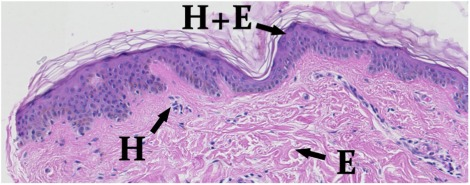
\includegraphics[scale=1.2]{images/HE-stain-example.jpg}
\caption{section of skin showing Hematoxylin(H) \& Eosin(E) stain interactions}
\label{fig:HE-fig}
\end{figure}

\subsection{Slide digitization}
Physical tissue slides are digitized using whole slide image scanners which contain an illumination system, an optical microscope and a focusing apparatus (\textit{\cite{ghaznavi2013digital}}). Scanners most commonly use Brightfield illumination (\textit{\cite{kino1996confocal}}) in which the entire tissue sample is uniformly illuminated. This works in conjunction with the H\&E staining to display the tissue as a dark coloured image on a white background making it easier to distinguish cellular structure. 

The final output of the slide scanner is a virtual rendering of the entire tissue slide, that can be viewed at resolutions of upto 0.25 \si{\micro\meter} corresponding to a 40x objective power of the scanning microscope. In order to replicate a slide under a microscope, WSIs exhibit a pyramid structure consisting of images at multiple resolutions. The base level stores the image in diagnostic resolution of a 40x objective, often containing 100,000 x 100,000 pixels (\textit{\cite{wang2012managing}}). As displayed in figure(\ref{fig:pyramid-fig}) The resolution is down sampled by a fixed factor at each subsequent level. The Cancer Genome Atlas program's repository contains WSIs with 4 resolution levels down-sampled with factors of 1.0, 4.0, 16.0 and 64.0. This feature of WSIs makes these images extremely bulky with average sizes around 1GB per image. 

\begin{figure}[h]
\centering
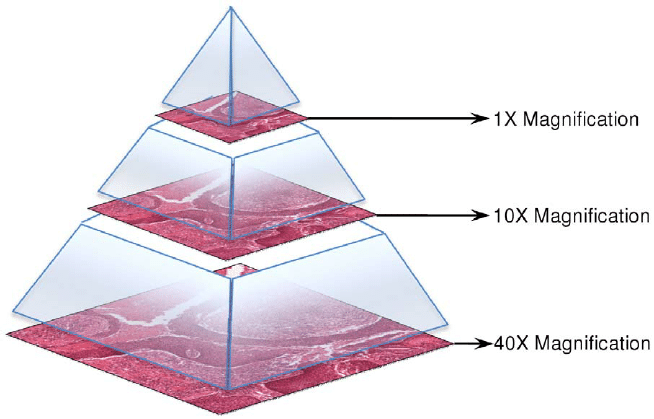
\includegraphics[scale=0.5]{images/digital-slide-stored-in-a-pyramid-structure.png}
\caption{Illustration of pyramid structure observed in whole slide images. Highest resolution at 40x magnification followed by 2 downsampled levels at 4.0 (10x) and 40.0 (1x)}
\label{fig:pyramid-fig}
\end{figure}

Viewing or analyzing an entire WSI is infeasible as the whole image simply cannot fit into a standard computer's memory. It was demonstrated by \cite{wang2012managing} that sectioning the WSI into several smaller, fixed size tiles at its diagnostic resolution and performing image analysis tasks on each tile allows for more efficient processing compared to using the entire slide image at once. As shown by \cite{aeffner2019introduction}, confining analysis efforts to smaller regions of interest (ROIs) rather than the entire WSI is often necessary to devise any accurate or computationally viable image analysis algorithms. The tile based results can be aggregated in order to generate masks that highlight all ROIs on lower resolution thumbnails of the original WSI in order to display the results of our image analysis tasks. 

\subsection{Slide normalization}
The manual preparation of tissue slides by pathologists is a very sensitive process and despite having an established staining protocol, several factors can imbue a high degree of variability in the presentation of the resulting WSI. As demonstrated by \cite{anghel2019high}, the lack of consistency in the quality and appearance of slide images is attributed to varying antigen concentration, temperatures at which the tissue is stored, physical conditions the slides are subjected to when being put through slide scanners and random human error involved in the process. \textbf{Figure \ref{fig:he-stain-difference}} illustrates how despite having a standardized staining procedure like the Hematoxylin \& Eosin staining, no two slides of the same tissue will exhibit identical color, stain intensity or physical structure.   

\begin{figure}[h]
\centering
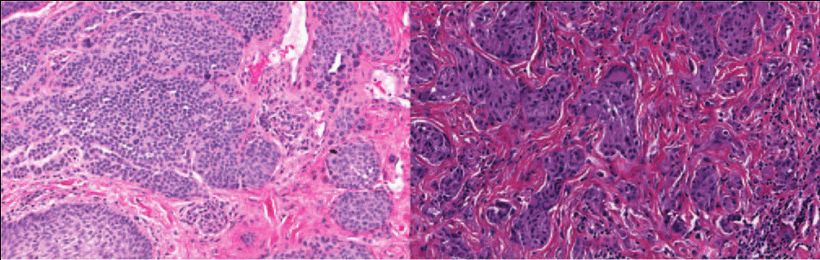
\includegraphics[scale=0.7]{images/stain-difference-slide.png}
\caption{Example of two H\&E stained whole slide images of melanomas obtained from different laboratories indicating the drastic difference in color appearance.}
\label{fig:he-stain-difference}
\end{figure}

\cite{li2015complete} establishes that performing any quantitative analysis on whole slide images requires numerical features obtained from an input image to be compared against features learned from prior training data. The disparities observed between the compared features help quantify any histopathological information conveyed by such images. If there exists additional variability in the WSI stemming from inconsistent slide preparation, then that corrupts the extracted features as they account for these non-histopathological differences and deviate from the true characterization of the sample. There is particularly high colour and intensity variation in slide images sourced from different pathology labs as each location has different conditions and personnel under which slides are produced. According to the paper on automated prostate cancer detection by \cite{gorelick2013prostate}, information conveyed by color variation on tissue samples is of extreme significance in the quantitative analysis of histopathological images. Therefore, it is crucial to achieve greater color consistency by implementing color normalization algorithms when working with models that utilize pattern recognition and color processing algorithms to deliver a diagnosis from learned features. 
\\

\subsection{Macenko method for color normalization}
The Macenko stain normalization method (\cite{macenko2009method}) is considered the gold standard for performing color normalization on H\&E stained whole slide images. This is evidenced by its application in a wide range of works such as, a paper on an end to end learning model for predicting tumour subtypes and genetic mutations from H\&E stained slide images by \cite{van2021deepmed}, predicting colorectal cancer from H\&E stained slides using deep learning by \cite{Kather2019} and \cite{anghel2019high} paper on robust stain normalization system for whole slide images. 

For slide images captured with standard RGB scanners, the stain absorbs three distinct wavelengths of light. \cite{macenko2009method} defines a \textit{stain vector} as the proportion of each wavelength absorbed by the staining component. The overall idea behind this normalization algorithm is that the color of a RGB pixel in a stained slide image is a linear combination of two stain vectors, corresponding to Hematoxylin (H) and Eosin (E). Being able to estimate these stain vectors effectively allows us to project each pixel onto any color plane, thereby converting the WSI into a standardized color profile. The Macenko stain normalization pipeline can be summarized as:
\begin{itemize}
    \item Applying a singular value decomposition (SVD) operation, approximate the H\&E stain vectors of all pixels inside the tissue sample (excluding white background pixels) in a given RGB slide image. 
    \item Apply an intensity correction operation to compensate for irregularities in stain concentration, quality of stain and staining protocol used by the original pathologist. 
    \item Project resulting image on a reference plane to ensure all normalized pixels exhibit a similar color profile. 
\end{itemize}
\hfill\\


\subsubsection{Macenko Algorithm}
\hfill\\
\cite{macenko2009method} prescribes the SVD based stain normalization algorithm as follows:\\
\\
\textbf{INPUT} : RGB slide image
\begin{itemize}
    \item Transform RGB slide to Opitcal Density (OD) form where \(OD = -\log_{10}(I)\), \(I\) being the RGB vector normalized to \([0.1]\).
    \item Remove pixels with OD intensity less than a pre-determined parameter \(\beta\). \cite{macenko2009method} proved \(\beta = 0.15\) provides the most robust normalization.
    \item Perform singular value decomposition on the OD tuples. Extract the two largest values by magnitude and generate the OD plane in their corresponding direction.
    \item Project input image data onto the resulting OD plane and normalize to unit length.
    \item Calculate \(\theta\), which is the angle of each point with respect to the direction of the \(1^{st}\) SVD value.
    \item Using pre-determined parameter \(\alpha\), calculate robust extremes of the angle which correspond to the \(\alpha^{th}\) and \((100 - \alpha)^{th}\) percentiles. \cite{macenko2009method} empirically recommends a value of \(\alpha = 1\) for the best normalization result. 
    \item Project extreme values back to OD space.
    \item Build optical density matrix (ODM) using the obtained projection from previous step
    \item Inverse ODM to estimate the respective concentration of the Hematoxylin and Eosin stains (\(C_h\) and \(C_e\)). 
    \item Determine the (\(100 - \alpha^{th}\)) percentile of \(C_h\) and \(C_e\).
    \item Upon transforming the normalized concentrations of each individual stain component to OD space, revert it back to RGB using an H\&E reference template. 
\end{itemize}


\begin{figure}[H]
\centering
\begin{tabular}{lccccc}
Raw slide image&
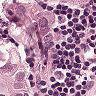
\includegraphics[width=80px]{images/37.jpeg}&
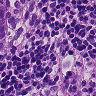
\includegraphics[width=80px]{images/68.jpeg}&
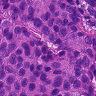
\includegraphics[width=80px]{images/195.jpeg}\\
After Macenko normalization&
 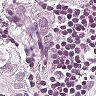
\includegraphics[width=80px]{images/37_macenko.jpeg}&
 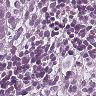
\includegraphics[width=80px]{images/68_macenko.jpeg}&
 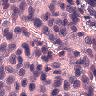
\includegraphics[width=80px]{images/195_macenko.jpeg}\\
 \\&
 (a)&(b)&(c)\\
\end{tabular}
\caption{Examples taken from training data - Illustrating effect of Macenko normalization on WSI patches of varying colour intensities }
\label{fig:macenko-example}
\end{figure}

\section{Deep Learning in histopathological analysis}
\subsection{Applications in WSI based diagnosis}
As proposed by \cite{gurcan2009histopathological}, diagnosing diseases from histopathological images requires the identification of some histological features, for example, cancer nuclei, glands or lymphocytes that serve as indicators of disease severity. With growing popularity of computer assisted diagnosis systems, Deep Learning has been proven to be the preferred approach for such classification and segmentation tasks on whole slide images. 

\cite{Kather2019} has proposed a supervised learning model that uses transfer learning to train a CNN that performs a patch based classification of nine tissue types observed in H\&E stained whole slide images of Colorectal cancer (CRC) samples. The study used 86 H\&E slides of CRC tissue to create a training set of image patches without any associated clinical data. The CNN was trained on these 224x224 px patches. They were labelled manually with patch-level annotations representing the relevant tissue class. The trained CNN would take a WSI, split it into 224x224 px patches and produce a prediction for the type of tissue a given patch represents with a unique color. Therefore, tile-level predictions were obtained to fully segment the given WSI into its constituent tissues and subsequently extract a deep-stromal score from the multi-class segmented WSI to determine the severity of CRC. 

A paper on detecting invasive ductal carcinoma (IDC) from whole slide images using a CNN was presented by \cite{cruz2014automatic}. As shown in figure \ref{fig:ductal-carcinoma-figure}, the paper proposes a supervised learning model trained using WSI patches containing patch-level annotations to learn a hierarchical  representation of malignant vs benign tissue. The CNN identifies tumour regions to determine tumour extent and severity and subsequently estimate disease prognosis. This deep learning based IDC region classification displayed a 84.23\% accuracy when compared to ground-truth pathologist annotations. The paper presents a comparison of the deep learning approach to more traditional machine learning classifiers implementing a Random Forest method for tumour classification using hand-crafted features like tumour area, texture, nuclear structure, color etc. Using a RGB histogram was only 77.24\% accurate while a fuzzy color histogram showed 78.74\% accuracy, proving the effectiveness of deep learning approaches when performing histopathological analysis. 

\begin{figure}[h]
    \centering
    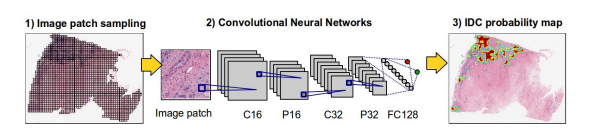
\includegraphics[scale=0.9]{images/Cruz-Roa-Ductal-Carcinoma-example.png}
    \caption{IDC detection framework from H\&E stained WSI - 1)Splitting WSI into tiles, 2)CNN outputs tile-level prediction for probability of being IDC positive, 3)Aggregate predicted tiles to show heatmap of most likely IDC regions with probability > 0.29}
    \label{fig:ductal-carcinoma-figure}
\end{figure}

The use of a patch/tile-based approach to train and segment WSIs is observed to be the most common technique to overcome the memory logistic issues associated with the large size and resolution of WSIs. An alternative approach to processing large WSI data was demonstrated by \cite{qin2018large} using a feature Pyramid method comprising of a ResNet50-GICN-GPP pipeline. The ResNet50 architecture was used as an encoder while combining the feature pyramid blocks as decoders which produced a segemntation accuracy of 63\% when tested on the CAMELYON16 challenge dataset. 

In the context of segmenting malignant breast tissue in H\&E stained WSIs, the paper by \cite{priego2020automatic} proposes a fast semantic segmentation pipeline. As observed in figure \ref{fig:Priego-conv-pipeline}, it performs tile-level segmentation of malignant or benign tissue using a DCNN along with a dilated convolutional encoder-decoder architecture. The paper prescribes using a pre-trained MobileNetV2 network as the backbone of the DCNN. The CNN's max pooling layer is replaced with the convolutional encoder to allow features to be extracted at any resolution, independent of the resolution of the input WSI. This makes it possible to accurately segment regions of the same tissue that may appear different due to scaling disparities in the input image compared to the training images. They applied a softmax function to the last layer of the CNN (as shown in figure \ref{fig:Priego-conv-pipeline}) in order to convert the discrete prediction (malignant vs benign) into tile-level probability maps. These probability maps were merged using a Conditional Random Field (CRF) method that allowed overlapping regions of tiles to be captured more efficiently without any loss of information. 

\begin{figure}[h]
    \centering
    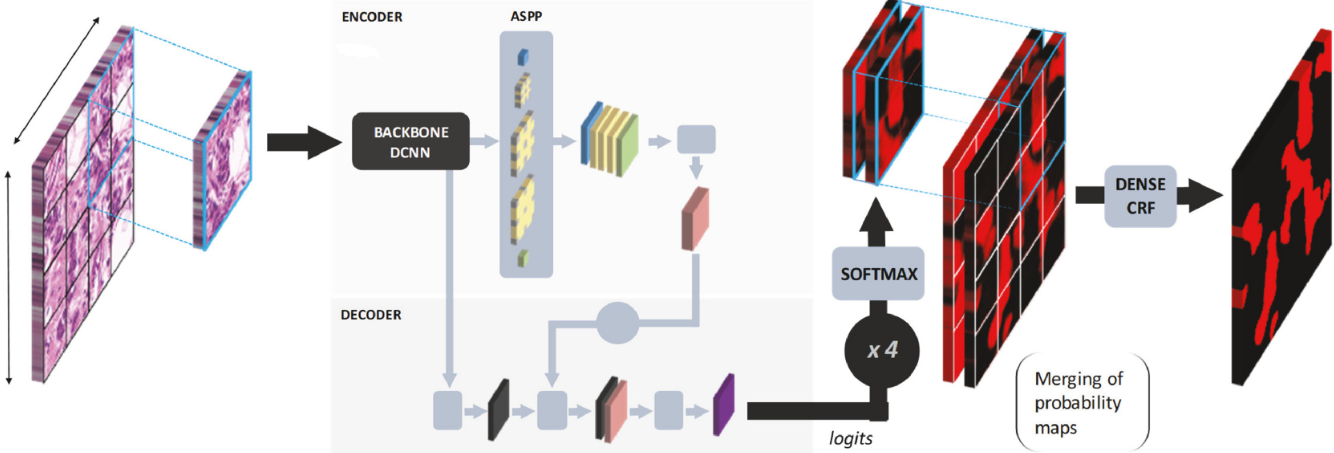
\includegraphics[scale=0.4]{images/Priego-DCNN-encoder-arch.png}
    \caption{\cite{priego2020automatic} - Tile-based semantic segmentation using DCNN and convolutional encoder to obtain probability maps of segmented tissue}
    \label{fig:Priego-conv-pipeline}
\end{figure}

\subsection{Methods to process WSI data for deep learning}
Whole slide images are captured at a minimum 40x magnification resulting in images having resolutions exceeding \(100,000 \times 100,000\) pixels with an average uncompressed size of 5GB (\cite{bandi2018detection}). Thus, a single image often exceeds the available memory size in most computers making it infeasible to perform tasks like patch extraction by loading the entire WSI to memory. This necessitates the use of specialized software to access such images and perform deep learning tasks such as extracting patches for patch-based tissue segmentation.

\cite{bankhead2017qupath} proposes a Java based whole slide processing tool called QuPath. It can be accessed through its own native GUI to perform WSI analysis but also supports Groovy scripts to execute high level algorithms such as patch extraction from WSIs. QuPath also provides the ability to build low level machine learning classifiers like Support Vector Machines or Random Forests within its integrated GUI environment. Recent developments with deep learning are yet to be translated into QuPath as it does not support  training CNNs natively and only allows predictions to be imported and viewed (\cite{pedersen2021fastpathology}). It is also very restrictive due to being a GUI and not having any API support for other languages. The GUI itself has a steep learning curve and is not very intuitive for users who are not experts/researchers in histopathology. 

\cite{goode2013openslide} have created Open Slide which is an open-source, vendor-neutral C library for viewing, processing and analyzing WSIs. The major problem in digital pathology is the lack of a standardized format for WSI. This causes WSI vendors to create their own proprietary format that requires their proprietary software to process. Open Slide aims to increase interoperability by facilitating transparent handling of various vendor formats of WSIs while supporting multiple programming language APIs. It offers a Python package to enable WSI processing through Python which makes it accessible for academic research.   

\subsection{Data availability for CNN training}
As reported in the paper on Colorectal Cancer diagnosis from histology slides by \cite{Kather2019}, all data used in training and validation of the CNN was manually annotated by an expert pathologist. They sectioned 86 CRC H\&E whole slides from the NCT biobank and UMM pathology archive to create a training set of 100,000 tiles. Each tile had to be manually annotated at a tile level. to describe the nine relevant tissue classes. Their validation set comprised of 862 H\&E slides retrieved from 500 CRC patients on The Cancer Genome Atlas (TCGA) repository. Data from TCGA does not contain any pixel or slide level annotations and had to be manually reviewed to identify relevant histological artifacts. 

\cite{priego2020automatic} further lay emphasis on the lack of publicly available H\&E stained whole slide images with strong pixel level annotations being a major hindrance in the development of supervised learning models. Their solution to this lack of annotated data was to create an OpenSlide based, online WSI viewer that allowed pathologists from across the world to view and hand annotate tumour regions, thereby constructing a training dataset tailored to this project for breast cancer lesion segmentation.

The CAMELYON16 and CAMELYON17 challenges were identified as viable data sources for training deep learning models to detect breast cancer metastases. \cite{Khened2021} proposed a generalized framework for WSI segmentation and validated its performance in breast cancer segmentation using CAMELYON16 and CAMELYON17 data. As shown by \cite{bejnordi2017diagnostic} in their paper on deep learning algorithms for breast metastases detection, the CAMELYON16 data serves as a very robust dataset for training supervised learning models as it contains 399 WSI (159 malignant and 240 benign samples), sourced from two separate laboratories with pixel level annotations of breast metastases found in sentinel lymph nodes. 

CAMELYON17 on the other hand was showcased by \cite{bandi2018detection} in assessing potential deep learning techniques for breast cancer detection and prognosis assessment. This dataset was built upon CAMELYON16 to include 1399 WSI of breast metastases in sentinel lymph node sections, sourced from five different laboratories to more accurately represent staining variability and allow for more robust training. Instead of pixel level annotations, CAMELYON17 included slide level annotations to allow for a shift of focus on patient-level diagnosis followed by patient prognosis prediction rather than diagnosing metastases in individual WSI. 
\\
\subsubsection{Why is CAMELYON data effective for diagnosing breast cancer?}
\hfill\\
The effectiveness of CAMELYON16 and CAMELYON17 data in diagnosing breast cancer despite containing lymph node biopsies is explained by \cite{sobin2011tnm} in their TNM staging system. In diagnosing breast cancer, clinicians consider the extent of tumour growth (T-stage), spreading of tumour cells to lymph nodes (N-stage) and the degree of metastases in other parts of the body (M-stage). Presence of breast metastatic cells in sentinel lymph nodes, which is the first lymph node breast cancer cells drain into, is therefore a significant indicator of breast cancer prognosis and can be used to learn how to characterize general breast metastases in deep learning models.


\section{Cancer prognosis estimation}
\subsection{Survival time analysis methods}
As an extension to deep learning based CRC diagnosis, \cite{Kather2019} have proposed fitting a uni-variable Cox-proportional Hazard model with features extracted from each tissue class to model their respective influence on patient-level survival prediction. Utilizing a Youden index \((sensitivity + specificity - 1)\), they determined an optimal Hazard Ratio (HR) cutoff value. All counts of tissue classes with HR > cutoff were weighted with their HR and combined to develop a deep stromal score quantifying slide-level disease severity. They propose a further step to fit a multivariate Cox proportional hazard model on the TCGA validation data, in order to adjust for clinical factors like tumour stage, sex and age when obtaining the Hazard Ratio. This multivariate HR showed higher confidence in prognosis predictions as it accounted for both slide-level tissue morphology and patient specific clinical factors. 

Other instances of survival analysis on histopathology images, such as the paper by \cite{Wetstein2022} illustrates a Kaplan-Meier survival analysis using a uni-variable and a multivariate Cox proportional hazard model. The multivariate analysis was included to produce more realistic survival predictions that accounted for clinical characteristics of each patient, such as current treatment, tumour dimensions and lymphovascular state. All these factors are ignored by the uni-variable model which only aims to utilize histological features in its prediction. A similar methodology was also proposed by \cite{Liu2022} using univariable Cox proportional hazard models. They having additionally demonstrated the use of Python's \textit{Lifelines} package in streamlining the Cox model fitting process and KM plot generation to visualize survival events. 

Majority of work in the field of automated survival estimation involves linear parametric Cox models as described previously. The applicability 
of these methods are constrained by the requirement of strong, pixel-level annotations in facilitating supervised learning models to extract precise features to successfully quantify survival. Alternate approaches of survival analysis are still being developed but are not as prominently established.  \cite{katzman2018deepsurv} proposed a feed-forward neural network called DeepSurv to quantify the influence of a patient's clinical and histological covariates on their hazard rate and subsequently support treatment recommendations. This method uses an alternate approach to  previously described linear Cox regression by using a neural network to optimize the partial likelihood loss function of the Cox model using non-linear features. \cite{wulczyn2020deep} illustrates another method of survival prediction using a weakly supervised learning approach. Uniformly sampled patches were drawn from the slides of a given patient, only knowing if the slide was malignant or benign. Image-based features extracted by the CNN from these patches were processed by a custom loss function - combination of cross-entropy and Cox partial likelihood loss - to output a probability distribution over discretized survival intervals for each patient.

\subsection{Cox proportional hazard model}
The original paper by \cite{cox1972regression}, demonstrated a generalized regression method as an extension to the Kaplan-Meier survival analysis approach. The Cox proportional hazard model is a linear regression model defined in terms of a hazard function (\(\lambda\)) as follows
\begin{equation}
    \centering
    \lambda (t | \textbf{x}) = \lambda_0 (t) \exp (\beta \textbf{x})
    \label{eq:hazard model}
\end{equation}

where \(t\) represents time, \textbf{\(x\)} denotes an \(n \times 1\) element vector of all covariates being modelled such that \(n=1\) for univariable Cox modelling and \(n > 1\) for multivariable models. \(\beta\) represents a vector of all regression coefficients in the model while \(\lambda_0 (t)\) denotes the baseline hazard under initial conditions of \(\textbf{x} = 0\). 

This hazard model displays the relation between the time until some event occurs (in survival models the event is the death of a subject) to the given covariates. The proportional nature of the model implies a multiplicative increase in hazard rate with unit increase in the covariate(s). This can be demonstrated by considering a univariable model where \(x\) and \(\beta\) are both one element vectors representing single covariate regression. Following a unit increase in the covariate, such that we have \(x + 1\) as our new covariate, the new hazard function is
\begin{equation}
    \centering
    \begin{aligned}
        \lambda (t | x + 1) ={}& \lambda_0 (t) \exp (\beta (x+1)) \\
                            ={}& \lambda_0 (t) \exp (x\beta  + \beta)) \\
                            ={}& (\lambda_0 (t) \exp (x\beta)) + \exp (\beta) \\
                            ={}& \lambda (t | x ) \exp (\beta)
    \end{aligned}
\end{equation}

denoting a constant multiplicative scaling by \(\exp (\beta)\) of our original hazard function upon a unit increase in covariate. Furthermore, upon changing sides of the new hazard function we get
\begin{equation}
    \centering
    \begin{aligned}
        \frac{\lambda (t | x + 1)}{\lambda (t | x )} = \exp (\beta) 
    \end{aligned}
\end{equation}

where the ratio \(\exp (\beta)\) is a constant with no time dependence. This represents the "proportional" nature of the Cox hazard model where the relationship over time between original and subsequent hazard functions remains constant despite changing covariates. 

\subsection{Kaplan-Meier analysis}
The Cox proportional hazard model only describes the hazard or probability of certain survival event happening at a specific point of time. It is useful in analyzing the risk of survival associated with given features. However, it cannot predict overall survival time as hazard is inversely proportional to survival, with survival showing rapid decline at high hazard function values. As defined by \cite{bewick2004statistics}, having survived until a given time \(t\), the hazard function \(\lambda (t)\) corresponds to the probability of dying at \(t\). Whereas, the KM survival function \(S(t)\), represents probability of surviving until time \(t\). \cite{schober2021kaplan} proposes using the Kaplan-Meier method for producing exact survival time predictions. Kaplan-Meier generates a parametric survival function that estimates the probability of patient surviving past a certain point of time. Showing overall survival time prediction using Kaplan-Meier graphs is the most common methodology as observed in all survival analysis papers such as \cite{Kather2019}, \cite{Liu2022} and \cite{Wetstein2022}.

\begin{figure}[h]
    \centering
    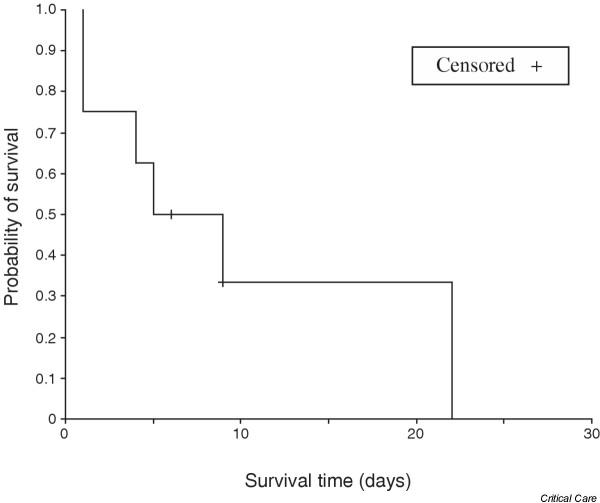
\includegraphics[scale=0.3]{images/KM-plot-example.jpg}
    \caption{\cite{bewick2004statistics} - Example Kaplan-Meier plot showing overall survival probability }
    \label{fig:km-plot-example}
\end{figure}

As observed in figure \ref{fig:km-plot-example}, a KM plot is a step-wise function plotting probability of survival on the y-axis and survival time in any discrete unit on the x-axis. KM plots can support multiple curves on the graph where each represent a unique covariate setting to see their influence on survival. The graph displays vertical drops in survival probability over time at points where an event of interest occurs, which in survival analysis is the death of a subject. The horizontal distance to these points on the curve represent the total interval of time after which the event occurred, thereby showing the probability a subject survives for that period of time. As proposed by \cite{bewick2004statistics}, the median survival time is often a good prediction of overall survival as it is the point of 0.5 probability where half the subjects perish and the other half lives. This median survival time can be used to compare multiple KM plots in terms of how severely  covariate influences survival.  

%==================================================================================================================================
\chapter{Analysis}
What is the problem that you want to solve, and how did you arrive at it?
\section{Guidance}
Make it clear how you derived the constrained form of your problem via a clear and logical process. 

%==================================================================================================================================
\chapter{Design}
How is this problem to be approached, without reference to specific implementation details? 
\section{Guidance}
Design should cover the abstract design in such a way that someone else might be able to do what you did, but with a different language or library or tool. 

%==================================================================================================================================
\chapter{Implementation}
What did you do to implement this idea, and what technical achievements did you make?
\section{Guidance}
You can't talk about everything. Cover the high level first, then cover important, relevant or impressive details.



\section{General points}

These points apply to the whole dissertation, not just this chapter.



\subsection{Figures}
\emph{Always} refer to figures included, like Figure \ref{fig:relu}, in the body of the text. Include full, explanatory captions and make sure the figures look good on the page.
You may include multiple figures in one float, as in Figure \ref{fig:synthetic}, using \texttt{subcaption}, which is enabled in the template.



% Figures are important. Use them well.
\begin{figure}
    \centering
    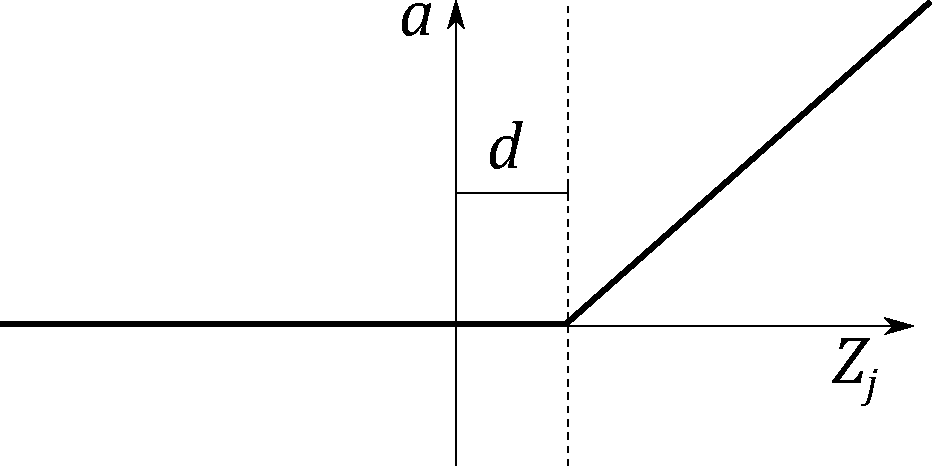
\includegraphics[width=0.5\linewidth]{images/relu.pdf}    

    \caption{In figure captions, explain what the reader is looking at: ``A schematic of the rectifying linear unit, where $a$ is the output amplitude,
    $d$ is a configurable dead-zone, and $Z_j$ is the input signal'', as well as why the reader is looking at this: 
    ``It is notable that there is no activation \emph{at all} below 0, which explains our initial results.'' 
    \textbf{Use vector image formats (.pdf) where possible}. Size figures appropriately, and do not make them over-large or too small to read.
    }

    % use the notation fig:name to cross reference a figure
    \label{fig:relu} 
\end{figure}


\begin{figure}
    \centering
    \begin{subfigure}[b]{0.45\textwidth}
        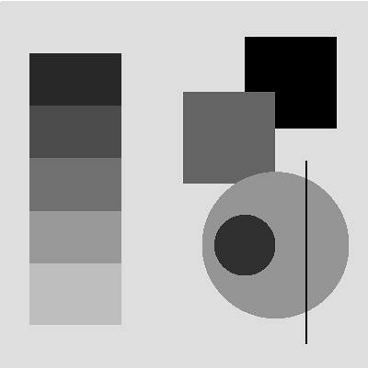
\includegraphics[width=\textwidth]{images/synthetic.png}
        \caption{Synthetic image, black on white.}
        \label{fig:syn1}
    \end{subfigure}
    ~ %add desired spacing between images, e. g. ~, \quad, \qquad, \hfill etc. 
      %(or a blank line to force the subfigure onto a new line)
    \begin{subfigure}[b]{0.45\textwidth}
        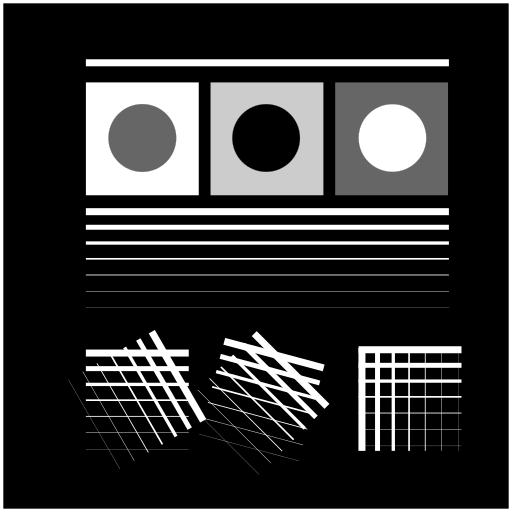
\includegraphics[width=\textwidth]{images/synthetic_2.png}
        \caption{Synthetic image, white on black.}
        \label{fig:syn2}
    \end{subfigure}
    ~ %add desired spacing between images, e. g. ~, \quad, \qquad, \hfill etc. 
    %(or a blank line to force the subfigure onto a new line)    
    \caption{Synthetic test images for edge detection algorithms. \subref{fig:syn1} shows various gray levels that require an adaptive algorithm. \subref{fig:syn2}
    shows more challenging edge detection tests that have crossing lines. Fusing these into full segments typically requires algorithms like the Hough transform.
    This is an example of using subfigures, with \texttt{subref}s in the caption.
    }\label{fig:synthetic}
\end{figure}

\clearpage

\subsection{Equations}

Equations should be typeset correctly and precisely. Make sure you get parenthesis sizing correct, and punctuate equations correctly 
(the comma is important and goes \textit{inside} the equation block). Explain any symbols used clearly if not defined earlier. 

For example, we might define:
\begin{equation}
    \hat{f}(\xi) = \frac{1}{2}\left[ \int_{-\infty}^{\infty} f(x) e^{2\pi i x \xi} \right],
\end{equation}    
where $\hat{f}(\xi)$ is the Fourier transform of the time domain signal $f(x)$.

\subsection{Algorithms}
Algorithms can be set using \texttt{algorithm2e}, as in Algorithm \ref{alg:metropolis}.

% NOTE: line ends are denoted by \; in algorithm2e
\begin{algorithm}
    \DontPrintSemicolon
    \KwData{$f_X(x)$, a probability density function returing the density at $x$.\; $\sigma$ a standard deviation specifying the spread of the proposal distribution.\;
    $x_0$, an initial starting condition.}
    \KwResult{$s=[x_1, x_2, \dots, x_n]$, $n$ samples approximately drawn from a distribution with PDF $f_X(x)$.}
    \Begin{
        $s \longleftarrow []$\;
        $p \longleftarrow f_X(x)$\;
        $i \longleftarrow 0$\;
        \While{$i < n$}
        {
            $x^\prime \longleftarrow \mathcal{N}(x, \sigma^2)$\;
            $p^\prime \longleftarrow f_X(x^\prime)$\;
            $a \longleftarrow \frac{p^\prime}{p}$\;
            $r \longleftarrow U(0,1)$\;
            \If{$r<a$}
            {
                $x \longleftarrow x^\prime$\;
                $p \longleftarrow f_X(x)$\;
                $i \longleftarrow i+1$\;
                append $x$ to $s$\;
            }
        }
    }
    
\caption{The Metropolis-Hastings MCMC algorithm for drawing samples from arbitrary probability distributions, 
specialised for normal proposal distributions $q(x^\prime|x) = \mathcal{N}(x, \sigma^2)$. The symmetry of the normal distribution means the acceptance rule takes the simplified form.}\label{alg:metropolis}
\end{algorithm}

\subsection{Tables}

If you need to include tables, like Table \ref{tab:operators}, use a tool like https://www.tablesgenerator.com/ to generate the table as it is
extremely tedious otherwise. 

\begin{table}[]
    \caption{The standard table of operators in Python, along with their functional equivalents from the \texttt{operator} package. Note that table
    captions go above the table, not below. Do not add additional rules/lines to tables. }\label{tab:operators}
    %\tt 
    \rowcolors{2}{}{gray!3}
    \begin{tabular}{@{}lll@{}}
    %\toprule
    \textbf{Operation}    & \textbf{Syntax}                & \textbf{Function}                            \\ %\midrule % optional rule for header
    Addition              & \texttt{a + b}                          & \texttt{add(a, b)}                                    \\
    Concatenation         & \texttt{seq1 + seq2}                    & \texttt{concat(seq1, seq2)}                           \\
    Containment Test      & \texttt{obj in seq}                     & \texttt{contains(seq, obj)}                           \\
    Division              & \texttt{a / b}                          & \texttt{div(a, b) }  \\
    Division              & \texttt{a / b}                          & \texttt{truediv(a, b) } \\
    Division              & \texttt{a // b}                         & \texttt{floordiv(a, b)}                               \\
    Bitwise And           & \texttt{a \& b}                         & \texttt{and\_(a, b)}                                  \\
    Bitwise Exclusive Or  & \texttt{a \textasciicircum b}           & \texttt{xor(a, b)}                                    \\
    Bitwise Inversion     & \texttt{$\sim$a}                        & \texttt{invert(a)}                                    \\
    Bitwise Or            & \texttt{a | b}                          & \texttt{or\_(a, b)}                                   \\
    Exponentiation        & \texttt{a ** b}                         & \texttt{pow(a, b)}                                    \\
    Identity              & \texttt{a is b}                         & \texttt{is\_(a, b)}                                   \\
    Identity              & \texttt{a is not b}                     & \texttt{is\_not(a, b)}                                \\
    Indexed Assignment    & \texttt{obj{[}k{]} = v}                 & \texttt{setitem(obj, k, v)}                           \\
    Indexed Deletion      & \texttt{del obj{[}k{]}}                 & \texttt{delitem(obj, k)}                              \\
    Indexing              & \texttt{obj{[}k{]}}                     & \texttt{getitem(obj, k)}                              \\
    Left Shift            & \texttt{a \textless{}\textless b}       & \texttt{lshift(a, b)}                                 \\
    Modulo                & \texttt{a \% b}                         & \texttt{mod(a, b)}                                    \\
    Multiplication        & \texttt{a * b}                          & \texttt{mul(a, b)}                                    \\
    Negation (Arithmetic) & \texttt{- a}                            & \texttt{neg(a)}                                       \\
    Negation (Logical)    & \texttt{not a}                          & \texttt{not\_(a)}                                     \\
    Positive              & \texttt{+ a}                            & \texttt{pos(a)}                                       \\
    Right Shift           & \texttt{a \textgreater{}\textgreater b} & \texttt{rshift(a, b)}                                 \\
    Sequence Repetition   & \texttt{seq * i}                        & \texttt{repeat(seq, i)}                               \\
    Slice Assignment      & \texttt{seq{[}i:j{]} = values}          & \texttt{setitem(seq, slice(i, j), values)}            \\
    Slice Deletion        & \texttt{del seq{[}i:j{]}}               & \texttt{delitem(seq, slice(i, j))}                    \\
    Slicing               & \texttt{seq{[}i:j{]}}                   & \texttt{getitem(seq, slice(i, j))}                    \\
    String Formatting     & \texttt{s \% obj}                       & \texttt{mod(s, obj)}                                  \\
    Subtraction           & \texttt{a - b}                          & \texttt{sub(a, b)}                                    \\
    Truth Test            & \texttt{obj}                            & \texttt{truth(obj)}                                   \\
    Ordering              & \texttt{a \textless b}                  & \texttt{lt(a, b)}                                     \\
    Ordering              & \texttt{a \textless{}= b}               & \texttt{le(a, b)}                                     \\
    % \bottomrule
    \end{tabular}
    \end{table}
\subsection{Code}

Avoid putting large blocks of code in the report (more than a page in one block, for example). Use syntax highlighting if possible, as in Listing \ref{lst:callahan}.

\begin{lstlisting}[language=python, float, caption={The algorithm for packing the $3\times 3$ outer-totalistic binary CA successor rule into a 
    $16\times 16\times 16\times 16$ 4 bit lookup table, running an equivalent, notionally 16-state $2\times 2$ CA.}, label=lst:callahan]
    def create_callahan_table(rule="b3s23"):
        """Generate the lookup table for the cells."""        
        s_table = np.zeros((16, 16, 16, 16), dtype=np.uint8)
        birth, survive = parse_rule(rule)

        # generate all 16 bit strings
        for iv in range(65536):
            bv = [(iv >> z) & 1 for z in range(16)]
            a, b, c, d, e, f, g, h, i, j, k, l, m, n, o, p = bv

            # compute next state of the inner 2x2
            nw = apply_rule(f, a, b, c, e, g, i, j, k)
            ne = apply_rule(g, b, c, d, f, h, j, k, l)
            sw = apply_rule(j, e, f, g, i, k, m, n, o)
            se = apply_rule(k, f, g, h, j, l, n, o, p)

            # compute the index of this 4x4
            nw_code = a | (b << 1) | (e << 2) | (f << 3)
            ne_code = c | (d << 1) | (g << 2) | (h << 3)
            sw_code = i | (j << 1) | (m << 2) | (n << 3)
            se_code = k | (l << 1) | (o << 2) | (p << 3)

            # compute the state for the 2x2
            next_code = nw | (ne << 1) | (sw << 2) | (se << 3)

            # get the 4x4 index, and write into the table
            s_table[nw_code, ne_code, sw_code, se_code] = next_code

        return s_table

\end{lstlisting}

%==================================================================================================================================
\chapter{Evaluation} 
How good is your solution? How well did you solve the general problem, and what evidence do you have to support that?

\section{Guidance}
\begin{itemize}
    \item
        Ask specific questions that address the general problem.
    \item
        Answer them with precise evidence (graphs, numbers, statistical
        analysis, qualitative analysis).
    \item
        Be fair and be scientific.
    \item
        The key thing is to show that you know how to evaluate your work, not
        that your work is the most amazing product ever.
\end{itemize}

\section{Evidence}
Make sure you present your evidence well. Use appropriate visualisations, reporting techniques and statistical analysis, as appropriate.

If you visualise, follow the basic rules, as illustrated in Figure \ref{fig:boxplot}:
\begin{itemize}
\item Label everything correctly (axis, title, units).
\item Caption thoroughly.
\item Reference in text.
\item \textbf{Include appropriate display of uncertainty (e.g. error bars, Box plot)}
\item Minimize clutter.
\end{itemize}

See the file \texttt{guide\_to\_visualising.pdf} for further information and guidance.

\begin{figure}
    \centering
    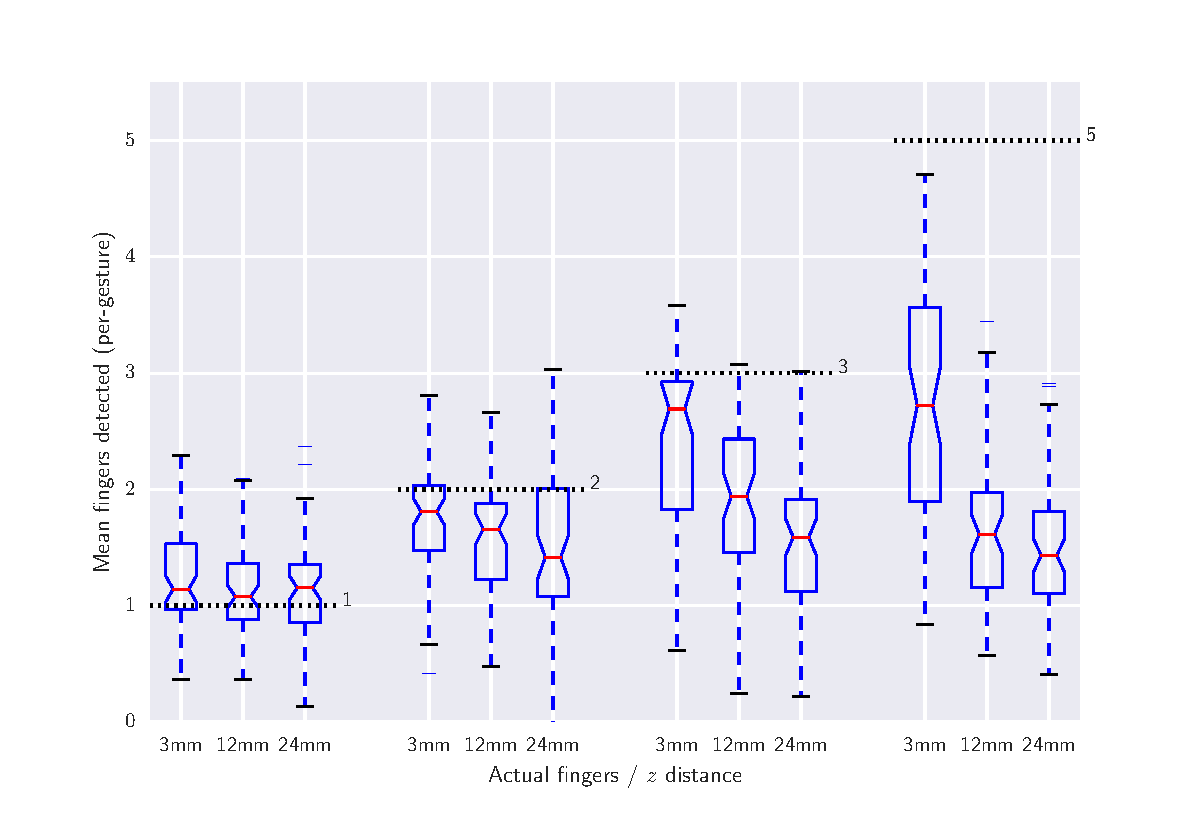
\includegraphics[width=1.0\linewidth]{images/boxplot_finger_distance.pdf}    

    \caption{Average number of fingers detected by the touch sensor at different heights above the surface, averaged over all gestures. Dashed lines indicate
    the true number of fingers present. The Box plots include bootstrapped uncertainty notches for the median. It is clear that the device is biased toward 
    undercounting fingers, particularly at higher $z$ distances.
    }

    % use the notation fig:name to cross reference a figure
    \label{fig:boxplot} 
\end{figure}


%==================================================================================================================================
\chapter{Conclusion}    
Summarise the whole project for a lazy reader who didn't read the rest (e.g. a prize-awarding committee).
\section{Guidance}
\begin{itemize}
    \item
        Summarise briefly and fairly.
    \item
        You should be addressing the general problem you introduced in the
        Introduction.        
    \item
        Include summary of concrete results (``the new compiler ran 2x
        faster'')
    \item
        Indicate what future work could be done, but remember: \textbf{you
        won't get credit for things you haven't done}.
\end{itemize}

%==================================================================================================================================
%
% 
%==================================================================================================================================
%  APPENDICES  

\begin{appendices}

\chapter{Appendices}

Typical inclusions in the appendices are:

\begin{itemize}
\item
  Copies of ethics approvals (required if obtained)
\item
  Copies of questionnaires etc. used to gather data from subjects.
\item
  Extensive tables or figures that are too bulky to fit in the main body of
  the report, particularly ones that are repetitive and summarised in the body.

\item Outline of the source code (e.g. directory structure), or other architecture documentation like class diagrams.

\item User manuals, and any guides to starting/running the software.

\end{itemize}

\textbf{Don't include your source code in the appendices}. It will be
submitted separately.

\end{appendices}

%==================================================================================================================================
%   BIBLIOGRAPHY   

% The bibliography style is abbrvnat
% The bibliography always appears last, after the appendices.

\bibliographystyle{apalike}

\bibliography{l4proj}

\end{document}
